\section{Descripción estructural con IP Catalog \label{sec:s2}}

\begin{center}
	\begin{minipage}{12cm}
		\begin{tcolorbox}[title=Actividad 2]
			Describir el multiplexor en forma estructural usando una función creada por el \textit{IP Catalog} siguiendo los pasos descritos en el documento o presentación. Simular el multiplexor.
		\end{tcolorbox}	
	\end{minipage}
\end{center}

Lo que se observa en la \autoref{fig:for_loop2_vhdl_rtl} es que se conectan de manera distinta los componentes del modulo. Al momento de compilar el proyecto se muestra un incremento significativo de las advertencias (Ver \autoref{fig:for_loop2_vhdl_warning}). Las simulaciones se visualizan en la \autoref{fig:for_loop2_vhdl_wavebi} en base binaria y en la \autoref{fig:for_loop2_vhdl_wavede} en base decimal, en donde se tiene que el resultado del producto punto es el valor ``X'' (conocido como ``no importa''), ya que no se inicializó la variable y cuando se realiza una operación aritmética con ``X'', el resultado siempre sera ``X''. Esto se comprueba con el mensaje que se observa en la \autoref{fig:for_loop2_vhdl_modelsim}.

\begin{figure}[ht]
	\centering
	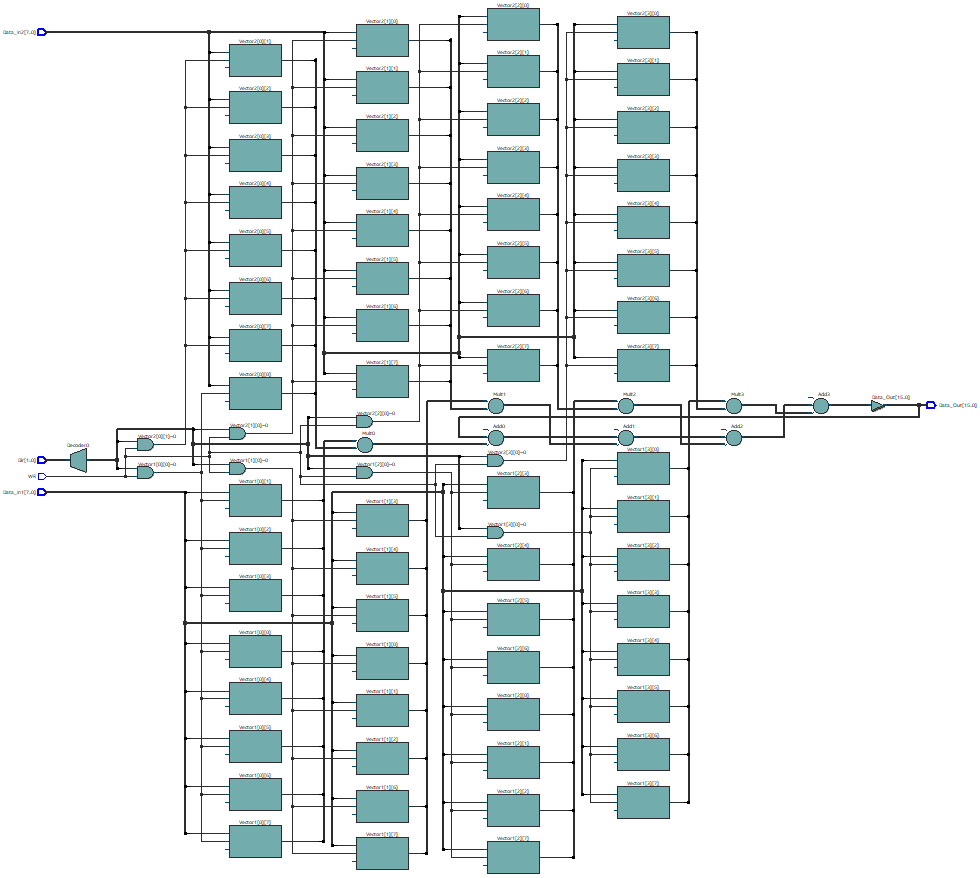
\includegraphics[scale=0.65]{For_Loop2_VHDL_RTL.png}
	\caption{Diagrama RTL del producto punto de dos vectores implementado en VHDL, sin inicializar la variable de suma de productos. \label{fig:for_loop2_vhdl_rtl}}
\end{figure}

\begin{figure}[ht]
	\centering
	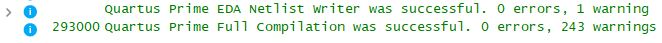
\includegraphics[scale=1]{For_Loop2_VHDL_Warning.png}
	\caption{Notorio incremento de los mensajes de advertencia al momento de compilar el proyecto debido a que la variable de suma de productos no se inicializó. \label{fig:for_loop2_vhdl_warning}}
\end{figure}

\begin{figure}[ht]
	\centering
	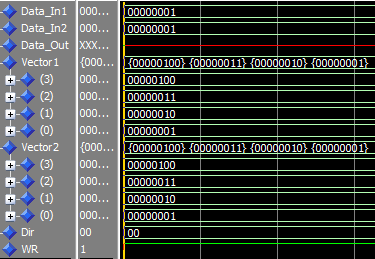
\includegraphics[scale=1.4]{For_Loop2_VHDL_WaveBi.png}
	\caption{Simulación del producto punto de dos vectores en VHDL, sin inicializar la variable de suma de productos, con el visor de formas de onda de ModelSim (base binaria). \label{fig:for_loop2_vhdl_wavebi}}
\end{figure}

\begin{figure}[ht]
	\centering
	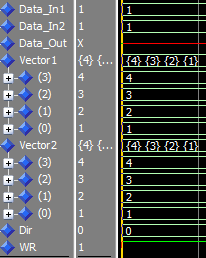
\includegraphics[scale=1.4]{For_Loop2_VHDL_WaveDe.png}
	\caption{Simulación del producto punto de dos vectores en VHDL, sin inicializar la variable de suma de productos, con el visor de formas de onda de ModelSim (base decimal). \label{fig:for_loop2_vhdl_wavede}}
\end{figure}

\begin{figure}[ht]
	\centering
	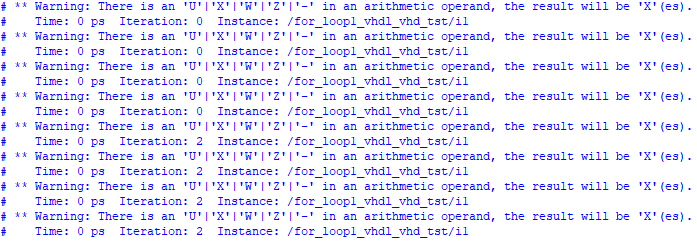
\includegraphics[scale=0.9]{For_Loop2_VHDL_ModelSim.png}
	\caption{Mensaje del simulador ModelSim debido a que la variable de suma de productos no se inicializó. \label{fig:for_loop2_vhdl_modelsim}}
\end{figure}